\documentclass[12pt,a4paper,twoside]{book}

\usepackage{FiraSans}
%\usepackage[default,regular,black]{sourceserifpro}
%\usepackage[extralight]{CrimsonPro}

\usepackage[11pt]{moresize}
\usepackage{anyfontsize}
\usepackage{t1enc}
\usepackage{mathptmx}
\usepackage{trace}
\usepackage{bookmark}
\usepackage{graphicx}
\usepackage{PTSerif}
\usepackage{epstopdf}
\usepackage{indentfirst}
\usepackage{verbatim}
\usepackage{amsthm}
\usepackage{amssymb}
\usepackage[list=true]{subcaption}
\usepackage{latexsym}
\usepackage{mathtools}
\usepackage{alphabeta}
\usepackage{listings}
\usepackage{scalerel}
\usepackage{stackengine}
\usepackage[explicit]{titlesec}
\usepackage[svgnames, tables]{xcolor}
\usepackage{float}
\usepackage{hyphenat}
\usepackage{tikz}
\usepackage{sectsty}
\usepackage{spverbatim}
\usepackage{fvextra}
\usepackage{afterpage}
\usepackage{xpatch}
\usepackage{pgfplots}
\usepackage{hyperref}
\usepackage{cleveref}       % improved cross referencing
\usepackage{textcomp}       % \textdegree = °C and other useful symbols
\usepackage{eurosym}
\usepackage{makeidx}
\usepackage{pdfpages}
\usepackage{circuitikz}
\usepackage{pbox}
\usepackage{yhmath}
\usepackage{tabularx}       % for ability to adjust column spacing in tabular better
\usepackage{booktabs}       % for better tables
\usepackage{etoolbox}
\usepackage{longtable}
\usepackage{csquotes}
\usepackage{filecontents}
\usepackage{framed}
\usepackage{titletoc}
\usepackage{booktabs}
\usepackage[inline]{enumitem}
\usepackage[normalem]{ulem}
\usepackage{mathrsfs}
\usepackage{epigraph}
\usepackage[breakable,most]{tcolorbox}
\usepackage{parskip}
\usepackage{nameref}
\usepackage{enumerate}
\usepackage{mathpazo}
\usepackage{ifoddpage}
\usepackage{textcomp}
\usepackage{textalpha}
\usepackage{array}
\usepackage{fancyhdr}
\usepackage{cmap}
\usepackage[Export]{adjustbox}
\usepackage{relsize}
\usepackage{grffile}
\usepackage{caption}
\usepackage{upquote}
\usepackage{charter}
\usepackage{eurosym}
\usepackage{enumitem}
\usepackage{blindtext}
\usepackage{calc}
\usepackage[subfigure]{tocloft}
\usepackage{footmisc}
\usepackage{mdframed}
\usepackage[section, newfloat]{minted}

\usepackage{colortbl}
\tcbuselibrary{skins}

\newcolumntype{Y}{>{\raggedleft\arraybackslash}X}
\newcolumntype{C}{>{\centering\arraybackslash}X}
\newcolumntype{S}{>{\hsize=.06\hsize}C}
\newcolumntype{B}{>{\hsize=.44\hsize}C}


\definecolor{mywhite}{RGB}{252,252,252}
\definecolor{mygrey}{RGB}{235,235,235}
\definecolor{myblue}{RGB}{8,43,84}

\tcbset{tab1/.style={fonttitle=\itshape\large,fontupper=\normalsize\sffamily,colback=mygrey,colframe=myblue,colbacktitle=mywhite,coltitle=black,center title,freelance}}


\newenvironment{code}{\captionsetup{type=listing}}{}
\SetupFloatingEnvironment{listing}{name=Code}

\makeatletter
\let\oldPYGdefault\PYGdefault
\def\PYGdefault#1#2{\hbox{\oldPYGdefault{#1}{#2}}\allowbreak{}}
\makeatother

\newmintedfile[cppcode]{cpp}{
	fontfamily=tt,
	linenos=true,
	numberblanklines=true,
	numbersep=5pt,
	gobble=0,
	frame=leftline,
	framerule=0.4pt,
	framesep=2mm,
	funcnamehighlighting=true,
	obeytabs=false,
	mathescape=true,
	samepage=false,
	showspaces=false,
	showtabs =false,
	texcl=false
}

\newcommand\Yuge{\fontsize{32}{38}\selectfont}
\newcommand\HUGER{\fontsize{26}{30}\selectfont}

\addtocontents{toc}{\protect\newpage}

\renewcommand{\cfttoctitlefont} % ToC title
             {\usefont{T1}{lmss}{b}{n}\selectfont\Yuge}
\renewcommand{\cftchapfont} % chapter titles
             {\usefont{T1}{qhv}{b}{n}\selectfont\HUGER}
\renewcommand{\cftsecfont} % section titles
             {\usefont{T1}{bch}{m}{n}\selectfont}
\renewcommand{\cftsubsecfont} % subsection titles
             {\usefont{T1}{bch}{m}{n}\selectfont}
\renewcommand{\cftchappagefont} % chapter page numbers
             {\usefont{T1}{bch}{b}{n}\selectfont}
\renewcommand{\cftsecpagefont} % section page numbers
             {\cftsecfont}
\renewcommand{\cftsubsecpagefont} % subsection page numbers
             {\cftsubsecfont}

\definecolor{myblue}{RGB}{8,43,84}
\definecolor{num}{RGB}{0,0,102}
\definecolor{sep}{RGB}{255,128,0}

\DeclarePairedDelimiter\ceil{\lceil}{\rceil}
\DeclarePairedDelimiter\floor{\lfloor}{\rfloor}

\usetikzlibrary{shapes,arrows,positioning,automata,intersections,shapes.misc,spy}

\newcommand{\ctikzlabel}[2]{\pbox{\textwidth}{#1\\#2}} % multiple-lines labels
\tikzset{
    pin/.style = {font = \relsize{-2}} % pin font size
}
\ctikzset{
    bipoles/length = 2em, % bipole size
    font = \relsize{-1}, % default font size
}

\let\Oldincludegraphics\includegraphics

\newcommand\YUGE{\fontsize{42}{50}\selectfont}

% Colors for the hyperref package
\definecolor{urlcolor}{rgb}{0,.145,.698}
\definecolor{citecolor}{rgb}{.12,.54,.11}
\adjustboxset{max size={0.9\linewidth}{0.9\paperheight}}

\hypersetup{
	pdftitle={Feed Forward Neural Network in C++ 17 and OpenMP for performance optimization},
	pdfauthor={Andreas Karatzas},
	pdfpagelabels=true,
	bookmarksnumbered=true,
	bookmarksopen=true,
	breaklinks=true,
	colorlinks=true,
	urlcolor=urlcolor,
	linktocpage=true,
	linkcolor=myblue,
	citecolor=citecolor,
	unicode=true
}

\newfontfamily\customfont{FiraGO}
\newfontfamily\hackfont{Roboto-Light}

\newcounter{nalg}[chapter] 									% defines algorithm counter for chapter-level
\renewcommand{\thenalg}{\thechapter .\arabic{nalg}} 		% defines appearance of the algorithm counter
\DeclareCaptionLabelFormat{algocaption}{Algorithm \thenalg} % defines a new caption label as Algorithm x.y

\lstnewenvironment{algorithm}[1][] 							%defines the algorithm listing environment
{
    \refstepcounter{nalg} %increments algorithm number
    \captionsetup{labelformat=algocaption,labelsep=colon} %defines the caption setup for: it ises label format as the declared caption label above and makes label and caption text to be separated by a ':'
    \lstset{ %this is the stype
        mathescape=true,
        frame=tB,
        numbers=left,
        numberstyle=\tiny,
        basicstyle=\scriptsize,
        keywordstyle=\color{black}\bfseries\em,
        keywords={,input, output, return, datatype, function, in, if, else, foreach, while, begin, end, } %add the keywords you want, or load a language as Rubens explains in his comment above.
        numbers=left,
        xleftmargin=.04\textwidth,
        #1 % this is to add specific settings to an usage of this environment (for instnce, the caption and referable label)
    }
}
{}

\DeclareMathOperator*{\argmax}{arg\,max}
\DeclareMathOperator*{\argmin}{arg\,min}

\DeclarePairedDelimiter\abs{\lvert}{\rvert}
\newcommand\reallywidesmile[1]{%
	\stackon[0.5pt]{#1}{%
		\stretchto{%
			\scaleto{%
				\scalerel*[\widthof{#1}]{\mkern-1.5mu\smile\mkern-2mu}%
				{\rule[-\textheight/2]{1ex}{\textheight}}%
			}{\textheight}%
		}{0.8ex}}%
}

\DeclareCaptionFormat{listing}{\rule{\dimexpr\textwidth+17pt\relax}{0.4pt}\par\vskip1pt#1#2#3}
\captionsetup[lstlisting]{format=listing,singlelinecheck=false, margin=0pt, font={sf},labelsep=space,labelfont=bf}
\renewcommand\lstlistingname{Code}

\newlength{\chaptertopskip}
\newlength{\chapterbottomskip}
\setlength{\chaptertopskip}{-30pt}
\setlength{\chapterbottomskip}{60pt}

\hyphenpenalty=1000
\emergencystretch=5em
\renewcommand\epigraphflush{flushleft}
\renewcommand\epigraphsize{\normalsize}

\makeatletter
\renewcommand\verbatim@font{\normalfont\fontencoding{T1}\ttfamily}
\makeatother

\setlength\epigraphwidth{0.7\textwidth}

\newenvironment{fname}{\fontfamily{lmtt}\selectfont}{\par}

\DeclareTextFontCommand{\filename}{\fname}

\newcommand\blankpage{%
	\null
	\thispagestyle{empty}%
	\addtocounter{page}{-1}%
	\newpage}

\let\emph\textit
\usepackage[top=3cm,bottom=3cm,left=3cm,right=3cm,headheight=22pt,headsep=25pt,heightrounded,footskip=1.5cm]{geometry}

\pagestyle{fancy}
\fancyheadoffset[LE,RO]{\marginparsep+\marginparwidth - 95pt}
\renewcommand{\chaptermark}[1]{\markboth{#1}{}}
\renewcommand{\sectionmark}[1]{\markright{ #1}}
\fancyhf{}
\fancyhead[RO]{\customfont\textbf{\nouppercase{Section \thesection{}}\quad\textcolor{myblue}{$\blacksquare$}\quad}\textit{\rightmark}\quad\quad\textcolor{sep}{\textbf\thepage}}
\fancyhead[LE]{\customfont\textcolor{sep}{\textbf\thepage}\textbf{\quad\quad\nouppercase{Chapter{ }\thechapter\quad\textcolor{myblue}{$\blacksquare$}\quad}}\textit{\leftmark}}
\fancypagestyle{plain}{%
\fancyhead{} % get rid of headers
\renewcommand{\headrulewidth}{0pt}
}

\newlength\ChapWd
\settowidth\ChapWd{\huge\chaptertitlename}

\titleformat{\chapter}[display]
  {\normalfont\filcenter\sffamily}
  {\tikz[remember picture,overlay]
    {
    \node[fill=myblue,font=\fontsize{60}{72}\selectfont\color{white},anchor=north east,minimum size=\ChapWd]
      at ([xshift=-15pt,yshift=-15pt]current page.north east)
      (numb) {\thechapter};
    %\node[rotate=90,anchor=south,inner sep=0pt,font=\huge] at (numb.west) {\chaptertitlename};
    }
  }{0pt}{\fontsize{33}{40}\selectfont\color{myblue}#1}
\titlespacing*{\chapter}
  {0pt}{10pt}{20pt}

\definecolor{MSBlue}{rgb}{.204,.353,.541}
\definecolor{MSLightBlue}{rgb}{.31,.506,.741}

\sectionfont{\normalfont\Large\bfseries\customfont}
\subsectionfont{\normalfont\Large\bfseries\customfont}

\renewcommand*{\footnotelayout}{\small\hackfont}

\makeatletter
\xpatchcmd{\ttl@printlist}{\endgroup}{{\noindent\color{myblue}\rule{\textwidth}{1.5pt}}\vskip30pt\endgroup}{}{}
\makeatother


\setlength\epigraphrule{0pt}
\renewcommand\textflush{flushright}
\renewcommand\epigraphsize{\normalsize\itshape}

% command for the circle for the number of part entries
\newcommand\Circle[1]{\tikz[overlay,remember picture]
  \node[draw,circle, text width=18pt,line width=1pt] {#1};}

% patching of \tableofcontents to use sans serif font for the tile
\patchcmd{\tableofcontents}{\contentsname}{\sffamily\contentsname}{}{}
% patching of \@part to typeset the part number inside a framed box in its own line
% and to add color
\makeatletter
\patchcmd{\@part}
  {\addcontentsline{toc}{part}{\thepart\hspace{1em}#1}}
  {\addtocontents{toc}{\protect\addvspace{20pt}}
    \addcontentsline{toc}{part}{\huge{\protect\color{sep}%
      \setlength\fboxrule{2pt}\protect\Circle{%
        \hfil\thepart\hfil%
      }%
    }\\[2ex]\color{num}\sffamily#1}}{}{}

\makeatother

\newenvironment{absolutelynopagebreak}
  {\par\nobreak\vfil\penalty0\vfilneg
   \vtop\bgroup}
  {\par\xdef\tpd{\the\prevdepth}\egroup
   \prevdepth=\tpd}

\setlength \epigraphwidth {\linewidth}
\setlength \epigraphrule {0pt}
\AtBeginDocument{\renewcommand {\epigraphflush}{center}}
\renewcommand {\sourceflush} {center}

% this is the environment used to typeset the chapter entries in the ToC
% it is a modification of the leftbar environment of the framed package
\renewenvironment{leftbar}
  {\def\FrameCommand{\hspace{6em}%
    {\color{sep}\vrule width 2pt depth 6pt}\hspace{1em}}%
    \MakeFramed{\parshape 1 0cm \dimexpr\textwidth-6em\relax\FrameRestore}\vskip2pt%
  }
 {\endMakeFramed}

% using titletoc we redefine the ToC entries for parts, chapters, sections, and subsections
\titlecontents{part}
  [0em]{\centering}
  {\contentslabel}
  {}{}
\titlecontents{chapter}
  [0em]{\vspace*{2\baselineskip}}
  {\parbox{4.5em}{%
    \hfill\Huge\sffamily\bfseries\color{num}\thecontentspage}%
   \vspace*{-2.3\baselineskip}\leftbar\textsc{\small\chaptername~\thecontentslabel}\\\sffamily}
  {}{\endleftbar}
\titlecontents{section}
  [8.4em]
  {\sffamily\contentslabel{3em}}{}{}
  {\hspace{0.5em}\nobreak\itshape\color{num}\contentspage}
\titlecontents{subsection}
  [8.4em]
  {\sffamily\contentslabel{3em}}{}{}
  {\hspace{0.5em}\nobreak\itshape\color{num}\contentspage}

\newtheorem{theorem}{Theorem}

\newcommand*{\fullref}[1]{\hyperref[{#1}]{\nameref*{#1}}}

\begin{document}
	\begin{titlepage}

	\newgeometry{left=11mm,right=11mm,top=50mm,bottom=0pt}
	\pagecolor{black}
	\color{black}

	\begin{tikzpicture}[remember picture,overlay]
	\node[anchor=north east,
	      xshift=-10mm,
	      yshift=-12mm]
	      at (current page.north east)
	      {
	        \color{white}
	        \begin{tabular}{r}
	        \textbf{\Large{ECBE Department}} \\[0.2cm]
	        \large{\emph{SIUC}} \\[0.085cm]
	        \normalsize{\today}
	        \end{tabular}
	      };
	\end{tikzpicture}

	\begin{center}
		\color{white}
	    \begin{flushleft}
	    	{\Yuge \bfseries ECE 572 - Neural Networks\\\vspace*{.4cm}\itshape Project}\\[0.7cm]
		 \vspace{0.4cm}

	    \end{flushleft}

	    \vspace{.012\textheight}

	    \begin{minipage}[t]{\textwidth}
	        \begin{flushleft} \large
	            \emph{Andreas Karatzas - 856523415}  \\[0.1cm]
	        \end{flushleft}
	    \end{minipage}
	    \vfill
	\end{center}


	% ECBE logo
	\begin{tikzpicture}[remember picture,overlay]
	\node[anchor=north west,
	      xshift=8.9mm,
	      yshift=-8.3mm]
	     at (current page.north west)
	     {
\includegraphics[width=.2\linewidth]{static/figures/saluki.png}};
	\end{tikzpicture}

	% Cover photo
	\begin{tikzpicture}[remember picture,overlay]
	\node[anchor=south, % anchor is bottom of picture
	      xshift=0pt,
	      yshift=-2.9mm] % shifting picture to actually be at the bottom of the page
	     at (current page.south) % placement at bottom of the page
	     {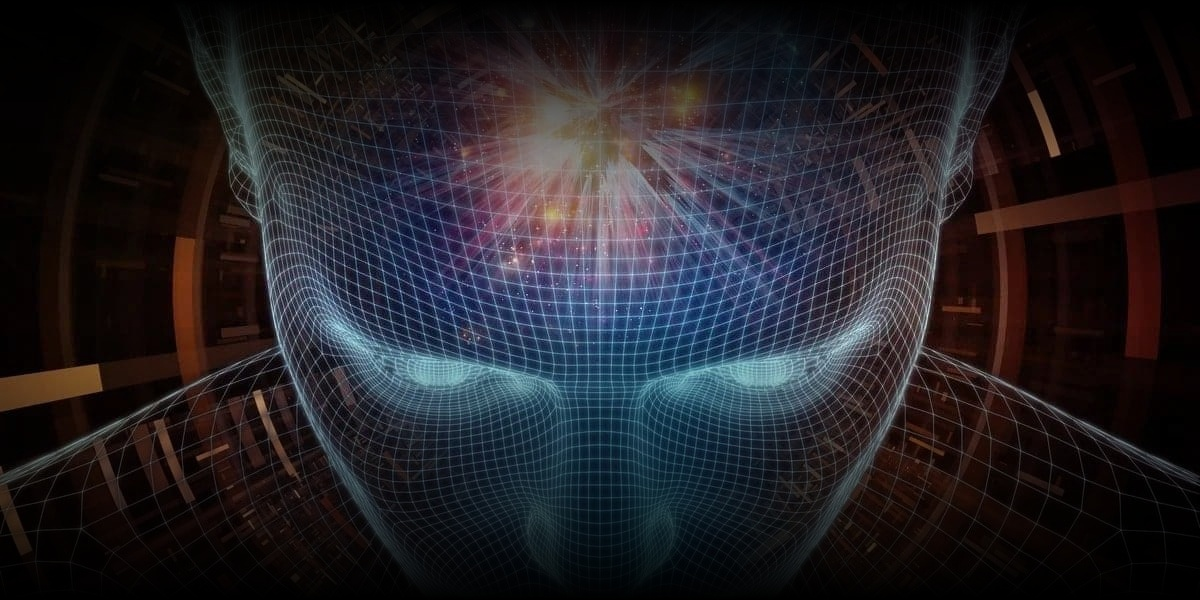
\includegraphics[height=18.9cm,keepaspectratio]{static/figures/cvBlurredOutput.jpg}};
	\end{tikzpicture}

	\end{titlepage}

	\pagecolor{white}

	\restoregeometry
	\pdfbookmark{\contentsname}{toc}
	\renewcommand{\baselinestretch}{1.5}\normalsize
	\begin{absolutelynopagebreak}
	\vspace{-2cm}
	\tableofcontents
	\end{absolutelynopagebreak}
	\renewcommand{\baselinestretch}{1.07}\normalsize

	
\chapter{Feed Forward Neural Network in C++ 17 and OpenMP for performance optimization}

\section{Abstract}


In the project for course ECE 572, I will implement a feed forward neural network with sigmoid activation function. 

\section{Introduction}

Artificial Neural Networks (ANNs) are used in wide range of applications including system modeling and identification, signal processing, image processing, control systems and time series forecasting. The baseline of those models is a special class called Feed Forward Neural Network\cite{bebis1994nns,murat2006overview}. In this subclass of models, data is propagated forward only, and the model parameters are grouped in layers with no intra-communication. There is theoretically an infinite number of possible architecture regarding this type of models, hence they can have a lot of layers. In fact, Feed Forward Neural Networks were the beginning of a new Artificial Intelligence (AI) sub-field called Deep Learning, where the models used are designed to capture complicated patters. For that purpose, the model architecture as well as the dataset used to train them is very large. Consequently, in such cases the model performance poses a substantial challenge. There are several attempts on efficient ANN implementation using techniques, such as parallelization, to exploit the computational capabilities of the system architecture running a model\cite{huqqani2013multicore}. Using low-level programming languages, such as C++\cite{stourstrup2013cpp}, and frameworks that enable advanced parallelization and efficient data handling techniques, such as OpenMP\cite{dagum1998openmp}, the programmer can achieve better results in terms of performance compared to most state-of-the-art Deep Learning frameworks\cite{Jang2008NeuralNI}. 

\par

For the project of course ECE 572, I will try to implement a feed forward model with sigmoid activation function. The user will have to make little to no configurations before the execution of the driver. It will be fully re-configurable regarding the architecture of the model. For example, the user will be able to define the layers and number of neurons using command line arguments. Moreover, the software architecture will follow that of well known deep learning frameworks, such as PyTorch\cite{paszke2019pytorch}. That way the user will be able to easily navigate around the project if there is some prior experience with such frameworks. Furthermore, the user will be kept well informed throughout the data loading, the training and the inference process with \textit{progress bars}. Finally, the advantages of the proposed project will be demonstrated using a well known dataset, Fashion MNIST\cite{FashionMNIST2017Xiao}.

\section{Challenges}

The implementation of a neural network in theory is an easy process. However, when it comes to putting together those formulas using software, the engineer is challenged to compile an efficient code implementation. The challenge becomes even greater when the project is carried out in a low-level programming language, such as C++, where the engineer has to solve substantial numerical and challenges since the project is based on scientific computation. After solving those challenges, the engineer has to structure the code in order to implement parallel software architectures and data pipelining for efficient execution. In this project, the optimization part will utilize the OpenMP framework for software parallelization and extreme device utilization.

    
    {
        \protect
        \bibliographystyle{ieeetr}
        \bibliography{refs.bib}
    }
\end{document}
